\documentclass[11pt]{article}
\usepackage[margin=2cm]{geometry}
\usepackage{booktabs}
\usepackage{graphicx}
\usepackage{xcolor}
\usepackage{enumitem}
\usepackage{parskip}
\usepackage{titlesec}
\usepackage{hyperref}
\hypersetup{colorlinks=true, urlcolor=blue!55!black}
\definecolor{teal}{HTML}{2A9D8F}
\definecolor{amber}{HTML}{E08A2E}
\titlespacing*{\section}{0pt}{8pt}{3pt}
\titleformat{\section}{\large\bfseries\color{black!82}}{}{0pt}{}
\titlespacing*{\subsection}{0pt}{5pt}{1pt}
\titleformat{\subsection}{\normalsize\bfseries}{}{0pt}{}
\setlist{nosep,leftmargin=1.4em}
\pagestyle{empty}
\newcommand{\code}[1]{\texttt{\small #1}}

\begin{document}
\sloppy

\begin{center}
{\LARGE\bfseries Two taxonomies for the building-block library}\\[2pt]
{\normalsize How each one is structured in the database, and how it was obtained \hfill \today}
\end{center}
\vspace{-2pt}\hrule\vspace{6pt}

\section*{Overview}
Every commercial building block in our library (\textbf{$\approx$1.95 million} unique molecules)
is described along two independent axes, kept as \textbf{separate layers} so that neither
constrains the other:
\begin{itemize}
  \item a \textbf{structural} taxonomy --- \emph{what each molecule is} (its chemical skeleton
        and functional groups);
  \item a \textbf{target} taxonomy --- \emph{what each molecule acts on} (the protein families it
        has measured activity against).
\end{itemize}
Both are organised as \textbf{rooted trees} (a single top node; every class has exactly one
parent), and both are stored in the same normalised shape: a \emph{nodes} table (one row per
class) plus an \emph{edges} table (one row per parent$\rightarrow$child link) --- the standard
adjacency-list representation of a hierarchy. Compound-to-class assignments live in \emph{separate}
fact tables, so the taxonomies themselves stay immutable and the assignment step is swappable.

\begin{figure}[h]
\centering
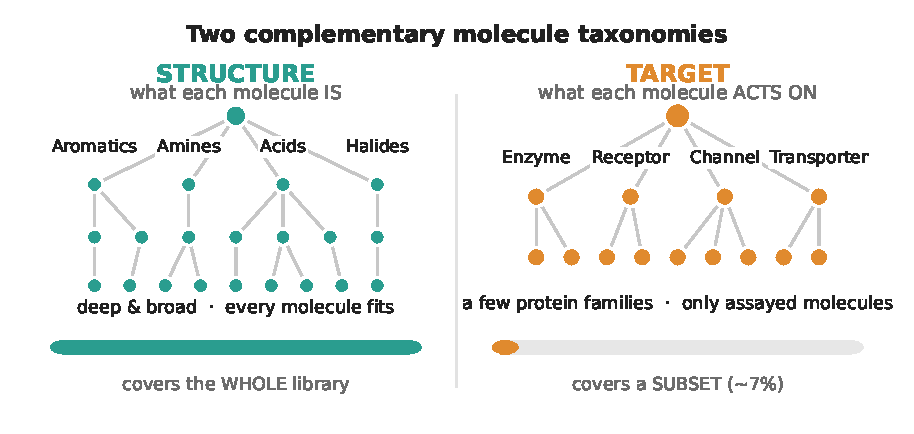
\includegraphics[width=0.96\linewidth]{figures/taxonomy_schematic.pdf}
\end{figure}

\section*{1. Structural taxonomy --- ChemOnt / ClassyFire}
\textbf{What it is.} ChemOnt is the reference chemical-structure classification used by the
ClassyFire system. It is a strict tree of \textbf{4{,}825 classes} under a single root
(\emph{Chemical entities}), \textbf{up to 11 levels} deep; the two top branches are
\emph{Organic} and \emph{Inorganic} compounds, which split into 31 broad superclasses and then
into progressively finer classes (e.g.\ \emph{Benzenoids $\rightarrow$ Benzene derivatives
$\rightarrow$ Benzonitriles}). It classifies structure only --- not biological activity.

\textbf{Database structure.} Stored as an adjacency list:
\code{chemont\_nodes} (\code{chemont\_id}, \code{name}, \code{definition}, \code{parent\_id},
\code{depth}) and \code{chemont\_edges} (\code{parent\_id}, \code{child\_id}); the full
root-to-leaf lineage of every class is precomputed in \code{chemont\_lineage.json}. Genuine
per-molecule labels are held separately in \code{classyfire\_ground\_truth} (each row: molecule
key, the kingdom/superclass/class/subclass/terminal it was assigned, the reconstructed lineage,
provenance, and an evidence level).

\textbf{How it was obtained.} (i) We parsed the canonical \code{ChemOnt\_2\_1.obo} ontology file
locally and verified its topology (single root, no multi-parent nodes, no cycles). (ii) We then
retrieved \textbf{genuine} classifications for the molecules by exact structural-key (InChIKey)
lookups against the authoritative ClassyFire services, over about two weeks of polite, automated
querying, caching every response. (iii) Every returned class identifier was validated against the
local ontology before being accepted. This produced \textbf{200{,}001} genuine labels spanning
26 superclasses, 425 classes and 1{,}977 terminal classes; a fast local rule-based predictor was
also benchmarked against them for the (larger) unlabelled remainder.

\section*{2. Target taxonomy --- ChEMBL protein classes}
\textbf{What it is.} A hierarchy of \emph{protein target families} from the ChEMBL bioactivity
database: a tree of \textbf{905 classes}, \textbf{6 levels} deep, under a single root
(\emph{Protein class}). Its top branches are broad functional groups --- \emph{Enzyme}
(e.g.\ kinase, protease, cytochrome P450), \emph{Membrane receptor} (e.g.\ GPCR families),
\emph{Ion channel}, \emph{Transporter}, \emph{Transcription factor}, \emph{Epigenetic
regulator} --- each refined into specific families. It classifies \emph{what a molecule binds},
not what it is.

\textbf{Database structure.} Same adjacency-list shape: \code{target\_class\_tree\_nodes}
(\code{class\_id}, \code{parent\_class\_id}, \code{pref\_name}, \code{class\_level}, and the full
path string) and \code{target\_class\_tree\_edges} (\code{parent\_class\_id},
\code{child\_class\_id}). The molecule-to-class assignments are held separately in
\code{target\_class\_layer\_enriched} (each row: molecule, the protein target it was assayed
against, and that target's class path \code{class\_l1 > class\_l2 > class\_l3}).

\textbf{How it was obtained.} The protein-family hierarchy is \emph{not} exposed by the ChEMBL web
API, so we downloaded the full \textbf{ChEMBL~37 SQLite release} locally and reconstructed the
tree by joining four of its tables:
\code{target\_dictionary} $\rightarrow$ \code{target\_components} $\rightarrow$
\code{component\_class} $\rightarrow$ \code{protein\_classification}. We then attached this tree
to our molecules through their measured bioactivities. Coverage is intrinsically limited: only
about \textbf{7\%} of the library has any recorded ChEMBL activity, and of the targets involved
$\approx$55\% carry a protein-family class (the rest are cell-lines, whole-organism or unchecked
screening targets). This layer is therefore an \emph{optional enrichment on a small, drug-like
subset}, not a library-wide backbone.

\section*{At a glance}
\begin{center}
\footnotesize
\setlength{\tabcolsep}{4pt}
\renewcommand{\arraystretch}{1.2}
\begin{tabular}{lll}
\toprule
 & \textbf{\textcolor{teal}{Structural (ChemOnt)}} & \textbf{\textcolor{amber}{Target (ChEMBL)}} \\
\midrule
answers & what the molecule \emph{is} & what it \emph{acts on} \\
shape & rooted tree & rooted tree \\
size / depth & 4{,}825 classes / 11 levels & 905 classes / 6 levels \\
root & Chemical entities & Protein class \\
coverage & whole library ($\approx$100\%) & a subset ($\approx$7\%) \\
source & ChemOnt 2.1 + ClassyFire & ChEMBL 37 dump \\
stored as & \code{chemont\_nodes/edges} & \code{target\_class\_tree\_*} \\
role & canonical backbone & optional facet \\
\bottomrule
\end{tabular}
\end{center}

\vspace{2pt}
{\footnotesize Both trees, the per-molecule assignments, and all code are in the project
repository (folder \code{database/v4/} for the trees, \code{reports/v4/} for documentation,
\code{scripts/v4/} for the code). The two layers are deliberately independent: the structural
taxonomy is the immutable backbone used everywhere, and the target taxonomy sits on top of it as
an optional, partial enrichment.}

\end{document}
